\begin{figure}[htb]
\centering
\begin{minipage}[c]{.45\linewidth}
\centering
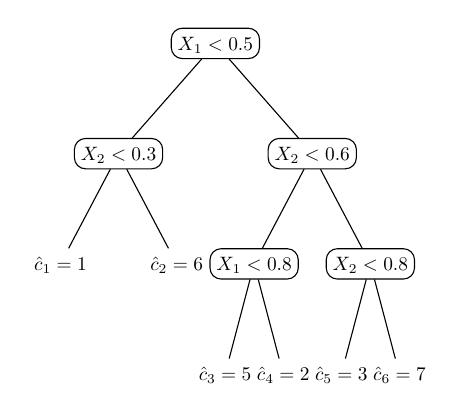
\begin{tikzpicture}[
scale = 0.7,
every node/.style={transform shape},
baseline,
level distance=20mm,
text depth=.1em,
text height=.8em,
level 1/.style={sibling distance=10em},
level 2/.style={sibling distance=6em},
level 3/.style={sibling distance=3em}]


	\node [rounded corners, draw] {$X_1 < 0.5$}
		child {node [rounded corners, draw] {$X_2 < 0.3$}
			child {node {$\hat{c}_1=1$}}
			child {node {$\hat{c}_2=6$}}
		}
		child {node [rounded corners, draw] {$X_2 < 0.6$}
			child {node [rounded corners, draw] {$X_1<0.8$}
				child {node {$\hat{c}_3=5$}}
				child {node {$\hat{c}_4=2$}}
			}
			child {node [rounded corners, draw] {$X_2<0.8$}
				child {node {$\hat{c}_5=3$}}
				child {node {$\hat{c}_6=7$}}
			}
	};

\end{tikzpicture}
\subcaption{Illustration Regression Tree}
\end{minipage}%
\hfill%
\begin{minipage}[c]{.45\linewidth}
\centering
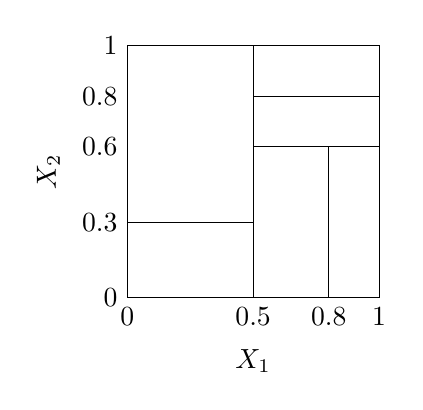
\begin{tikzpicture}[scale = 0.8]

\draw (0,0) -- (4,0) -- (4,4) -- (0,4) -- (0,0);
\draw (2,0) -- (2,4);
\draw (0,1.2) -- (2,1.2);
\draw (2,2.4) -- (4,2.4);
\draw (2,3.2) -- (4,3.2);
\draw (3.2,0) -- (3.2,2.4);
\node [left] at (0,0) {0};
\node [left] at (0,1.2) {0.3};
\node [left] at (0,2.4) {0.6};
\node [left] at (0,3.2) {0.8};
\node [left] at (0,4) {1};
\node [below] at (2,0) {0.5};
\node [below] at (0,0) {0};
\node [below] at (4,0) {1};
\node [below] at (3.2,0) {0.8};
\node[rotate=90] at (-1.25,2) {$X_2$};
\node at (2,-1) {$X_1$};
\end{tikzpicture}
\subcaption{Illustration Partition}
\end{minipage}
\caption[Illustration of a Regression Tree and its corresponding Partition]{Illustration of a Regression Tree and its corresponding Partition}
\label{fig:Tree_FigTreePar}

\end{figure}
